\chapter{Preliminaries}
\label{chap:background}

In this chapter, we will present definitions and primary results from the paper of 
Kriesell and Mohr \cite{matthias_2022}, which we will use to build up our investigations.

They introduced the concept of \textit{routing graphs} to more formally characterize the problem from the previous chapter, as we saw. 
First, let us define the transversal of a set partition, and then we can define the routing graph.

\begin{defn}[Transversal of a partition]
 A (minimal) \emph{transversal} of a \emph{partition} is a set containing exactly one
 element from each partition member and nothing else.
\end{defn}

\begin{example}
 Coloring $\mathfrak{C}$ of a graph partitions its vertices into color classes. 
 A transversal $T$ of this partition would contain exactly one vertex of each color from $\mathfrak{C}$.
\end{example}

\begin{defn}[Routing Graph]
Let $\mathfrak{C}$ be a coloring of graph $G$, let $T$ be the transversal of coloring $\mathfrak{C}$, 
then the \emph{routing graph} $H(G, \mathfrak{C}, T)$ is the graph with vertex set $T$,
where for every pair of vertices $u,v$ from $T$, $uv$ edge exists if and only if
there is a Kempe chain between $u$ and $v$ in $G$.
\end{defn}

Now, we can define the problem in a more compact way, which is as follows:

Which graphs $H$ have the property that, if $H$ is a
routing graph of some graph $G$ with coloring $\mathfrak{C}$ and a transversal $T$, then G
has $H$ as $T$-rooted minor? We say those graphs are \textit{KM-forcing}.

\section{KM-forcing graphs}

\begin{defn}[KM-forced]
    A graph $H$ is \emph{KM-forced} in graph $G$ if for every coloring $\mathfrak{C}$ of $G$ and transversal $T$ such that $H$ is isomorphic to the routing graph $H(G, \mathfrak{C}, T)$, the graph $G$ has $H(G, \mathfrak{C}, T)$ as a $T$-rooted minor.  
\end{defn}

\begin{defn}[KM-forcing]
 A graph $H$ is \emph{KM-forcing} if $H$ is KM-forced in every graph $G$.
\end{defn}

\begin{rem}
 The term \emph{KM-forcing} can be interpreted in two ways: as \emph{Kriesell–Mohr forcing} or as \emph{Kempe chain rooted minor forcing}. We leave the choice of interpretation to the reader's imagination.
\end{rem}

\begin{example}
    $K_1$ is KM-forcing. If $K_1$ is a routing graph $H(G, \mathfrak{C}, T)$, then $|T| = 1$, and $G$
can be colored with only one color; hence, it has no Kempe chains to other colored vertices, and $K_1$ is a rooted minor of $G$.
\end{example}

\begin{example}
 The complete graph $K_2$ is KM-forcing. 
 For any graph $G$ with coloring $\mathfrak{C}$ and transversal $T = \{u,v\}$ where the routing graph $H(G, \mathfrak{C}, T)$ is
 isomorphic to $K_2$, by definition there exists a Kempe chain between $u$ and $v$ in $G$. 
 Contracting all internal vertices of this chain while keeping $u$ and $v$ results in $uv$ edge. In the contracted graph of $G$,
 removing all unnecessary edges and vertices would result in $K_2$ as a rooted minor of $G$.
\end{example}

We will list several results from \cite{matthias_2022}, which capture properties of KM-forcing graphs. Moreover, they are helpful 
for later proofs. All the theorems in this chapter are proved in \cite{matthias_2022}.

\begin{thm}
\label{thm:1}
 If graph $H$ is KM-forcing, all its subgraphs are also KM-forcing.
\end{thm}

Theorem \ref{thm:1} is crucial for later showing that $K_7$ is not KM-forcing. It is sufficient to find a subgraph 
of $K_7$ which is not KM-forcing, and by theoerm \ref{thm:1} this would imply that $K_7$ is not KM-forcing as well.

Now, we will see a characterization of KM-forcing graphs, which helps to show that $K_4$ is KM-forcing.

\begin{thm}
\label{thm:1.5}
 Graph $H$ is KM-forcing if and only if every component of $K$ is KM-forcing.
\end{thm}

Another valuable result for further investigations is that a KM-forcing graph is still KM-forcing if we attach a pending edge to it.

\begin{thm}
\label{thm:2}
 Let $K$ be a graph and $q$ be a vertex with a degree of one. If $K - q$ is KM-forcing, then $K$ is KM-forcing as well.
\end{thm}


\section{Kempe chains and rooted $K_7$-minors}

\begin{defn}
 A coloring $\mathfrak{C}$ is a \emph{Kempe coloring} if any two vertices from distinct color classes belong 
 to the same Kempe chain. 
\end{defn}

Hadwiger \cite{hadwiger_1943} asked whether for a given Kempe coloring $\mathfrak{C}$ of a graph $G$ and transversal $T$, the graph $H:= H(G, \mathfrak{C}, T)$ is a complete graph 
and whether $G$ contains a $T$-rooted $H$ minor. This would follow if every complete graph were KM-forcing. 
By Theorem \ref{thm:1}, this would imply that \textit{every} graph is KM-forcing. 
It would prove Hadwiger's conjecture for graphs admitting Kempe colorings if true. 
However, as we will see, KM-forcing is too restrictive a property—and it already fails for $K_7$.

\begin{thm}\label{thm:3}
$K_7$ is not KM-forcing.
\end{thm}

By Theorem \ref{thm:1}, if $K_7$ were KM-forcing, all its subgraphs would also be KM-forcing. Thus, finding a subgraph of $K_7$ that is not KM-forcing is enough.

To construct graphs that are not KM-forcing, we need a graph $G$ with:
\begin{enumerate}
\item Enough paths between transversal vertices to form a routing graph
\item Not many edges incident to transversal vertices so that the construction of a rooted minor fails.
\end{enumerate}

A good construction with these properties is the \textit{$Z(H)$} graph:

\begin{defn}[$Z(H)$]
\label{defn:zg}
For a graph $H$, \emph{$Z(H)$} is defined as:
    \begin{enumerate}
        \item \textbf{Vertices:} $V(Z(H)) := V(H) \times \{1, 2\}$ \\
 Example: If $V(H):= \{a, b\}$, then $V(Z(H)):= \{(a,1), (b,1), (a,2), (b,2)\}$

        \item \textbf{Edges:} 
 For each edge $(x,y)$ from $E(H)$, the graph $Z(H)$ contains edges $((x,2)(y,2)), ((x,1)(y,2)),
 ((x,2)(y,1))$. \\
 Formally: \[ E(Z(H)) := \{(x,i)(y,j) : xy \in E(H) \text{ and } (i \neq 1 \text{ or } j \neq 1)\} \]
    \end{enumerate}
 Z(H) has coloring $\mathfrak{C} := \{\{(x,1),(x,2)\} : x \in V(H)\}$, and transversal $T := V(H) \times \{1\}$.

\end{defn}


Kriesell and Mohr found a subgraph $H$ of $K_7$ (Figure \ref{Fig:counterexample}) where the graph $Z(H)$ (Figure \ref{Fig:Main}) with coloring $\mathfrak{C}$ and transversal $T$ defined as above. 
They showed that $H$ is isomorphic to $H(Z(H), \mathfrak{C}, T)$, but $H$ is not a $T$-rooted minor of $Z(H)$.

\begin{figure}[H]
    \centering
    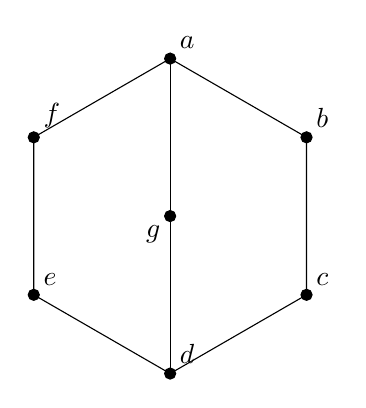
\begin{tikzpicture}[scale=1]

        \coordinate (a) at (0,2);
        \coordinate (b) at ({2*cos(30)},{2*sin(30)});
        \coordinate (c) at ({2*cos(-30)},{2*sin(-30)});
        \coordinate (d) at (0,-2);
        \coordinate (e) at ({2*cos(-150)},{2*sin(-150)});
        \coordinate (f) at ({2*cos(150)},{2*sin(150)});
        \coordinate (g) at (0,0);
        
        \draw (a) -- (b) -- (c) -- (d) -- (e) -- (f) -- cycle;
        
        \draw (g) -- (a);
        \draw (g) -- (d);
        
        \foreach \i in {a,b,c,d,e,f}{
            \filldraw (\i) circle (2pt);
            \node[above right] at (\i) {${\i}$};
 }
        
        % Draw x
        \filldraw (g) circle (2pt);
        \node[below left] at (g) {$g$};
        
        \end{tikzpicture}
        \caption{The subgraph of $K_7$ which is not KM-forcing}
        \label{Fig:counterexample}
\end{figure}




\begin{figure}[H]
    \centering
    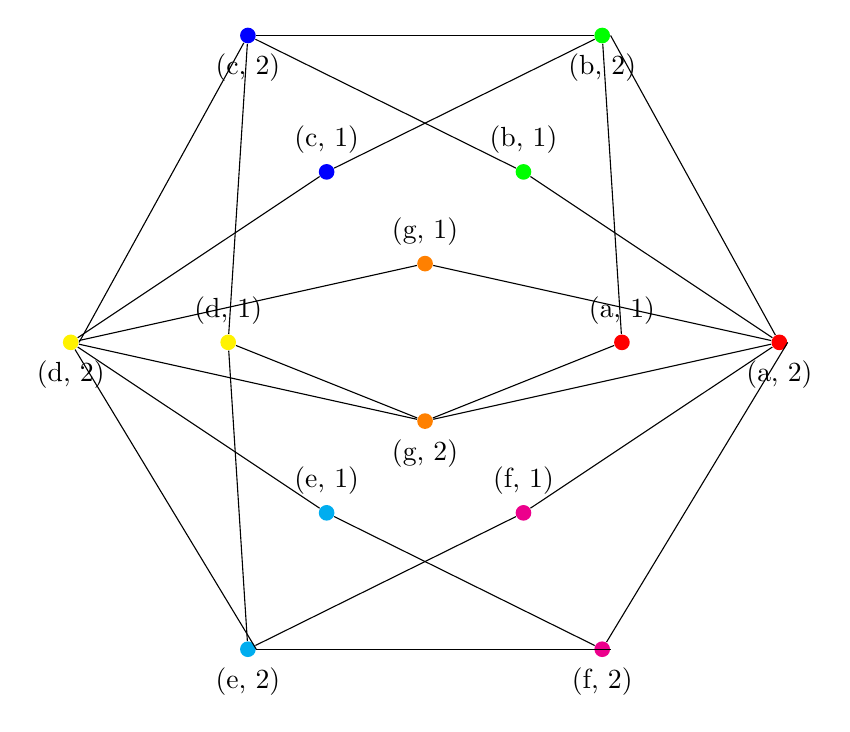
\begin{tikzpicture}
        \def\radius{2.5cm}
        \def\outerradius{4.5cm}
        
        % Add the central vertices (g, 1) and (g, 2) with the same color (orange)
        \node[circle, fill=orange, inner sep=2pt, label=above:{(g, 1)}] (vcenter1) at (0, 1) {}; % Shifted slightly up
        \node[circle, fill=orange, inner sep=2pt, label=below:{(g, 2)}] (vcenter2) at (0, -1) {}; % Shifted slightly down
        
        % Draw the inner circle vertices
        \foreach \i/\color [count=\j from 0] in {(a, 1)/red, (b, 1)/green, (c, 1)/blue, (d, 1)/yellow, (e, 1)/cyan, (f, 1)/magenta} {
            \node[circle, fill=\color, inner sep=2pt, label=above:\i] (v1\j) at ({360/6 * \j}:\radius) {};
 }
        
        % Draw the outer circle vertices
        \foreach \i/\color [count=\j from 0] in {(a, 2)/red, (b, 2)/green, (c, 2)/blue, (d, 2)/yellow, (e, 2)/cyan, (f, 2)/magenta} {
            \node[circle, fill=\color, inner sep=2pt, label=below:\i] (v2\j) at ({360/6 * \j}:\outerradius) {};
 }
        
        % Connect outer circle vertices
        \foreach \j in {0,...,5} {
            \pgfmathsetmacro{\nextj}{mod(\j+1, 6)}
            \draw (v2\j) -- (v2\nextj);
 }
        
        % Connect inner and outer circle vertices
        \draw (v20) -- (v11);
        \draw (v21) -- (v10);
        \draw (v22) -- (v11);
        \draw (v23) -- (v12);
        \draw (v21) -- (v12);
        \draw (v22) -- (v13);
        \draw (v24) -- (v13);
        \draw (v23) -- (v14);
        \draw (v25) -- (v14);
        \draw (v24) -- (v15);
        \draw (v20) -- (v15);
        
        % Connect (g, 2) to (a, 2) and (d, 2)
        \draw (vcenter2) -- (v20); % (g, 2) to (a, 2)
        \draw (vcenter2) -- (v23); % (g, 2) to (d, 2)
        
        % Connect (g, 1) to (a, 2) and (d, 2)
        \draw (vcenter1) -- (v20); % (g, 1) to (a, 2)
        \draw (vcenter1) -- (v23); % (g, 1) to (d, 2)
        
        % Connect (a, 1) to (g, 2) and (d, 1) to (g, 2)
        \draw (v10) -- (vcenter2); % (a, 1) to (g, 2)
        \draw (v13) -- (vcenter2); % (d, 1) to (g, 2)
    \end{tikzpicture}
    \caption{The graph $Z(H)$ given $H$ is the graph from \ref{Fig:counterexample}}
    \label{Fig:Main}
\end{figure}
In Figure \ref{Fig:Main}, the graph $Z(H)$ is shown with coloring and transversal described 
in the definition of Z(H) \ref{defn:zg}. For clarity, the transversal $T$ is the following $T:= \{(a, 1), (b, 1), (c, 1), (d, 1), (e, 1), (f, 1), (g, 1)\}$. \newline

\comment{I haven't done the computational part yet for the cases with $k = 7$ that we discussed before.}

We may be tempted to use the construction of \( Z(H) \) to check whether any graph $H$ is KM-forced in $Z(H)$. 
However, Kriesell and Mohr showed that for any graph \( H \) with at most six vertices, \( Z(H) \) always contains a \( T \)-rooted minor, where $T$ is the transversal of 
the coloring of $Z(H)$. 

\begin{thm}\label{thm:zg-for-k_6}
 Let $H$ be any graph with at most six vertices. Consider $Z(H)$ with coloring
    $\mathfrak{C}$ and the transversal $T$, as it's defined in \ref{defn:zg}. Then $Z(H)$ has a 
 $T$-rooted $H(Z(H), \mathfrak{C}, T)$-minor.
\end{thm}


There are also positive results, one of which is that $K_4$ is KM-forcing.

\begin{thm}\label{thm:6}
Every graph on at most four vertices is KM-forcing.
\end{thm}

One might ask whether the class of KM-forcing graphs is bounded. 
This is not the case, as implied by:

\begin{thm}\label{thm:4}
Every connected graph with at most one cycle is KM-forcing.
\end{thm}

As we can see, there is a gap between $K_4$ and $K_7$. We know that $K_4$ is KM-forcing and $K_7$ is not. What about the $K_5$ and $K_6$? The question for both of them is open, but there is a partial result on graphs with five 
vertices, which are the following:

\begin{thm}\label{thm:5}
Every graph on five vertices with at most six edges is KM-forcing.
\end{thm}

This result naturally leads us to the question of what happens when we consider graphs beyond this bound. 
In the next chapter, we will look into graphs \( G \), colorings $\mathfrak{C}$ and transversals
$T$ where some graph \( H \) which has at least five vertices and 
seven edges appears as the routing graph \( H(G, \mathfrak{C}, T) \) but is not a rooted minor of \( G \).